\section{Related work}
Here is short list of tools that fit this use case:
\begin{itemize}
    \item Repo-Visualizer \cite{repovisualizer} is a project that comes closest to this idea. It is an open-source tool that offers an interactive interface for visualizing and understanding repositories' structure, history, and collaboration dynamics. Key features include file tree visualization, commit history graphs, branch representation, and contributor analysis.

    \begin{figure}[!htbp]
        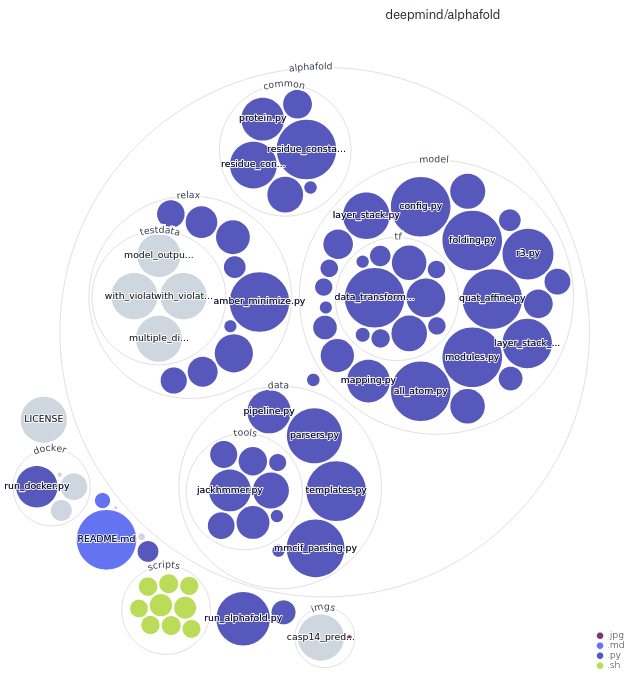
\includegraphics[width=8cm]{figs/repo-visualizer_sample.png}
        \centering
        \caption{Visualization produced by Repo-Visualizer}
        \small
        Repo Visualizer uses a tree like structure where files and directories are represented as circles. The circles of the members of a certain directory will lie within the circle of that directory as shown in the figure.
        \label{fig:repo-visualizer}
    \end{figure}

    \item Gource \cite{gource} is a visualization tool for source control repositories. The repository is displayed as a tree where the root of the repository is the centre, directories are branches and files are leaves. Contributors to the source code appear and disappear as they contribute to specific files and directories. Figure \ref{fig:gource} shows a visualization produced by gource of the Yum project \cite{yum}.

    \begin{figure}[!htbp]
        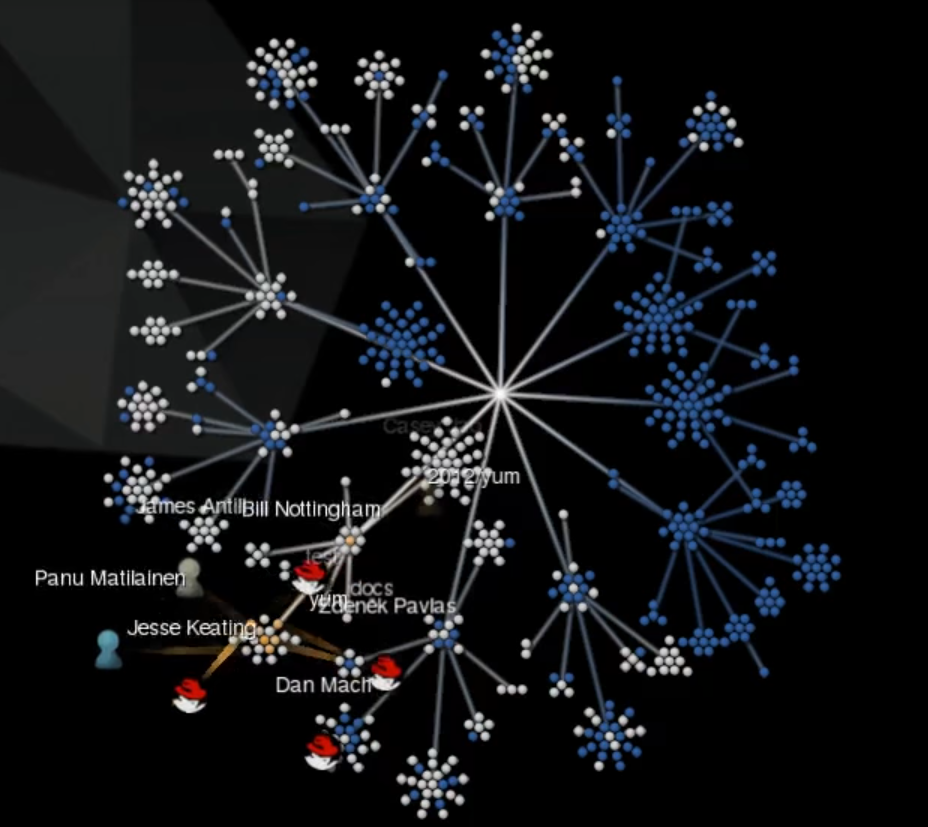
\includegraphics[width=8cm]{figs/gource_sample.png}
        \centering
        \caption{Gource Visualization}
        \small
        The image showcases Gource's unique visualization of the Yum project's \cite{yum} commit history. The visualization appears as a tree-like structure with branches representing directories and nodes representing files. Commits are displayed as animated actions performed by avatars representing the contributors.
        \label{fig:gource}
    \end{figure}
  
    \item GitKraken \cite{gitkraken} is a cross-platform Git client with a visual interface for managing repositories, including commit history graphs, branch visualization, and more. It also supports GitFlow, a branching model that streamlines collaboration and release management.
  
    \item Sourcegraph \cite{sourcegraph} is a web-based tool that indexes code from various version control systems, such as Git, and provides a search engine that supports advanced search queries, including regular expressions, filters, and search scopes. While Sourcegraph's primary focus is on code search and navigation, it does provide some visualization features such as dependency graphs but is not the main focus. 

    \item Additional work includes: Sourcetree \cite{sourcetree}, Github Desktop \cite{github_desktop}, GitLens \cite{gitlens}, etc.
\end{itemize}

